% !TEX program = xelatex
% AY2024 材料力学 解答例（同志社 生命医科学 医工学コース 院試）
% 問題・図は 01_exams/2024/tex を土台に、参考/ の粒度で解答を付した。
\documentclass[11pt,a4paper]{article}
\usepackage{../../00_common/preamble}
\usetikzlibrary{positioning,arrows.meta,calc,patterns,decorations.pathmorphing}

\title{材料力学 AY2024 解答例}
\author{}
\date{}

\begin{document}
\maketitle

\noindent\textbf{符号規約}：軸力・応力は引張りを正とする．はりの座標 $x$ は固定端 A から右向きにとり，
たわみ $v$ は下向きを正とする．たわみの基礎式は $EI\,\dfrac{d^2v}{dx^2}=M(x)$ を用い，
曲げモーメント $M$ は下に凸（さがり）を正とする．丸棒の断面二次モーメントを $I=\dfrac{\pi d^4}{64}$，
断面二次極モーメントを $J=\dfrac{\pi d^4}{32}$ とする．

%====================================================================
\section*{〔I〕}

図1に示すように, 断面積 $2A$, 縦弾性係数 $E$, 長さ $L$ の棒\textcircled{1}と, 断面積 $A$, 縦弾性係数 $3E$,
長さ $2L$ の棒\textcircled{2}からなる段付き棒の上端が天井に固定され, 下端に受皿が取り付けられている.
図1 (a) では質量 $m$ のリング状のおもりを受皿の上に静置した場合, 図1 (b) では同じおもりを $h$ の位置
まで持ち上げて静かに落下させた場合を考える. 各棒・受皿の重さは無視し, 重力加速度を $g$ とする.

\begin{center}
% (a)
\begin{tikzpicture}[>=Latex,scale=0.9,baseline=(current bounding box.north)]
  \node[above] at (0,6.2) {(a)};
  \fill[pattern=north east lines] (-1.3,6) rectangle (1.3,6.3); \draw (-1.3,6) -- (1.3,6);
  \draw (-0.7,4.5) rectangle (0.7,6.0);
  \draw (-0.35,1.5) rectangle (0.35,4.5);
  \draw[line width=1.2pt] (-1.0,1.5) -- (1.0,1.5);
  \fill (-0.95,1.5) rectangle (-0.4,2.0);
  \fill (0.4,1.5) rectangle (0.95,2.0);
  \node at (0,5.25) {棒\textcircled{1}}; \node at (0,3.0) {棒\textcircled{2}};
  \node[left] at (-0.95,2.3) {おもり}; \node[below] at (0,1.45) {受皿};
  \draw[<->] (1.05,4.5) -- (1.05,6.0) node[midway,fill=white]{$L$};
  \draw[<->] (1.05,1.5) -- (1.05,4.5) node[midway,fill=white]{$2L$};
\end{tikzpicture}
\hspace{14mm}
% (b)
\begin{tikzpicture}[>=Latex,scale=0.9,baseline=(current bounding box.north)]
  \node[above] at (0,6.2) {(b)};
  \fill[pattern=north east lines] (-1.3,6) rectangle (1.3,6.3); \draw (-1.3,6) -- (1.3,6);
  \draw (-0.7,4.5) rectangle (0.7,6.0);
  \draw (-0.35,1.5) rectangle (0.35,4.5);
  \draw[line width=1.2pt] (-1.0,1.5) -- (1.0,1.5);
  \fill (-0.95,3.0) rectangle (-0.4,3.5);
  \fill (0.4,3.0) rectangle (0.95,3.5);
  \node[left] at (-0.95,3.8) {おもり}; \node[below] at (0,1.45) {受皿};
  \node at (0,5.25) {棒\textcircled{1}}; \node at (0,2.2) {棒\textcircled{2}};
  \draw[<->] (-1.15,1.5) -- (-1.15,3.0) node[midway,fill=white]{$h$};
  \draw[<->] (1.05,4.5) -- (1.05,6.0) node[midway,fill=white]{$L$};
  \draw[<->] (1.05,1.5) -- (1.05,4.5) node[midway,fill=white]{$2L$};
\end{tikzpicture}

\vspace{1mm}
図1
\end{center}

\begin{enumerate}[label=(\arabic*)]
  \item 図1 (a) で棒\textcircled{1}と棒\textcircled{2}に生じる応力 $\sigma_1$, $\sigma_2$ を求めよ.
  \item 図1 (a) で段付き棒全体の伸び $\lambda$ を求めよ.
  \item 図1 (b) で生じる最大応力 $\sigma'_1$, $\sigma'_2$ について, 位置エネルギーとひずみエネルギーの
        間に成立する関係を $\sigma'_1$, $\sigma'_2$ で示せ.
  \item 図1 (b) の最大応力 $\sigma'_1$, $\sigma'_2$ を求めよ.
\end{enumerate}

\subsection*{解答}

\noindent\textbf{(1)}\quad 2本の棒は直列に接続され, おもりの重さ $W=mg$ を共通の軸力として受ける（引張）.
各棒の応力は軸力を断面積で割って
\[
  \sigma_1 = \frac{mg}{2A},\qquad \sigma_2 = \frac{mg}{A}.
\]
\[
  \ans{\;\sigma_1 = \dfrac{mg}{2A},\qquad \sigma_2 = \dfrac{mg}{A}\;}
\]
検算：軸力は $\sigma_1\cdot 2A = mg$, $\sigma_2\cdot A = mg$ でいずれも $mg$ に等しい ✓．

\medskip
\noindent\textbf{(2)}\quad 各棒の伸びは $\delta=\dfrac{N\ell}{(\text{断面積})\times(\text{縦弾性係数})}$ で与えられる．
\[
  \lambda_1 = \frac{mg\,L}{2A\,E},\qquad
  \lambda_2 = \frac{mg\,(2L)}{A\,(3E)} = \frac{2mgL}{3AE}.
\]
全体の伸びは両者の和で
\[
  \lambda = \frac{mgL}{2AE} + \frac{2mgL}{3AE}
          = \left(\frac{3}{6}+\frac{4}{6}\right)\frac{mgL}{AE}.
\]
\[
  \ans{\;\lambda = \dfrac{7mgL}{6AE}\;}
\]
検算：$\dfrac{1}{2}+\dfrac{2}{3}=\dfrac{7}{6}$ ✓．

\medskip
\noindent\textbf{(3)}\quad 落下衝撃では, おもりが受皿に達してから段付き棒が最大変形 $\lambda'$ を生じるまでの間,
おもりは合計 $h+\lambda'$ だけ降下する．このとき失われる位置エネルギー $mg(h+\lambda')$ が,
段付き棒に蓄えられるひずみエネルギー $U$ に等しい．\\
2本の棒は共通の軸力を受けるから $\sigma'_1\cdot 2A = \sigma'_2\cdot A$, すなわち
\[
  \sigma'_2 = 2\sigma'_1 .
\]
最大変形は各棒のひずみ $\times$ 長さの和であり
\[
  \lambda' = \frac{\sigma'_1}{E}\,L + \frac{\sigma'_2}{3E}\,(2L)
           = \frac{\sigma'_1 L}{E} + \frac{2\sigma'_2 L}{3E}.
\]
ひずみエネルギーは各棒で $U=\dfrac{\sigma'^2}{2(\text{縦弾性係数})}\times(\text{体積})$ より
\[
  U = \frac{\sigma'^2_1}{2E}\,(2A L) + \frac{\sigma'^2_2}{2(3E)}\,(A\cdot 2L)
    = \frac{\sigma'^2_1 A L}{E} + \frac{\sigma'^2_2 A L}{3E}.
\]
したがって成立する関係は
\[
  \ans{\;mg\!\left(h + \dfrac{\sigma'_1 L}{E} + \dfrac{2\sigma'_2 L}{3E}\right)
        = \dfrac{\sigma'^2_1 A L}{E} + \dfrac{\sigma'^2_2 A L}{3E}\;}
\]

\medskip
\noindent\textbf{(4)}\quad (3) の関係に $\sigma'_2 = 2\sigma'_1$ を代入する．
\[
  \lambda' = \frac{\sigma'_1 L}{E} + \frac{2(2\sigma'_1)L}{3E} = \frac{7\sigma'_1 L}{3E},
  \qquad
  U = \frac{\sigma'^2_1 A L}{E} + \frac{(2\sigma'_1)^2 A L}{3E} = \frac{7\sigma'^2_1 A L}{3E}.
\]
エネルギー保存 $mg(h+\lambda')=U$ は
\[
  mg\left(h + \frac{7\sigma'_1 L}{3E}\right) = \frac{7\sigma'^2_1 A L}{3E}
  \;\Longrightarrow\;
  A\,\sigma'^2_1 - mg\,\sigma'_1 - \frac{3Emgh}{7L} = 0.
\]
$\sigma'_1>0$ の根をとると
\[
  \sigma'_1 = \frac{mg + \sqrt{(mg)^2 + \dfrac{12AEmgh}{7L}}}{2A}
            = \frac{mg}{2A}\left(1 + \sqrt{1 + \frac{12AEh}{7mgL}}\,\right).
\]
\[
  \ans{\;\sigma'_1 = \dfrac{mg}{2A}\left(1 + \sqrt{1 + \dfrac{12AEh}{7mgL}}\,\right),\qquad
        \sigma'_2 = 2\sigma'_1 = \dfrac{mg}{A}\left(1 + \sqrt{1 + \dfrac{12AEh}{7mgL}}\,\right)\;}
\]
検算：衝撃応力は静的応力 $\sigma_1=\dfrac{mg}{2A}$ に衝撃係数
$\Bigl(1+\sqrt{1+2h/\lambda}\,\Bigr)$ を乗じたものに等しい．
ここで静たわみは (2) の $\lambda=\dfrac{7mgL}{6AE}$ で,
$\dfrac{2h}{\lambda}=\dfrac{12AEh}{7mgL}$ となり上式の根号内と一致する ✓．

%====================================================================
\clearpage
\section*{〔II〕}

図2のように, 点 A で固定された長さ $2L$ の丸棒（直径 $d$）の中央点 C に曲げモーメント $M_C$,
端点 B に集中荷重 $P$ とトルク $T_B$ が作用している. 丸棒の縦弾性係数を $E$, 横弾性係数を $G$ とする.
点 D は A から $L/2$ の位置にある.

\begin{center}
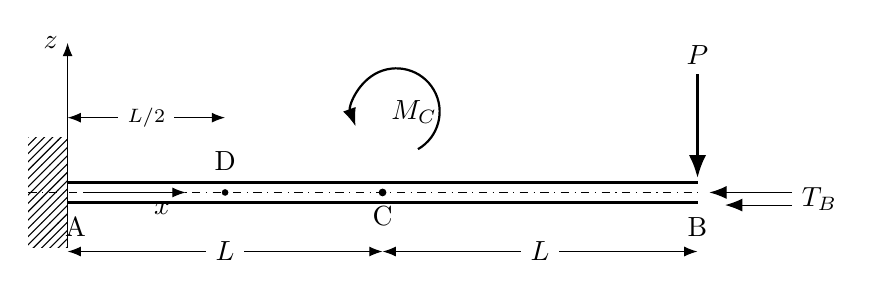
\begin{tikzpicture}[>=Latex]
  \fill[pattern=north east lines] (-0.5,-0.7) rectangle (0,0.7); \draw (0,-0.7) -- (0,0.7);
  \draw[line width=1.2pt] (0,0.13) -- (8,0.13);
  \draw[line width=1.2pt] (0,-0.13) -- (8,-0.13);
  \draw[dash dot] (-0.5,0) -- (8.0,0);
  \draw[->] (0,0) -- (0,1.9) node[left]{$z$};
  \draw[->] (0.2,0) -- (1.5,0); \node[below] at (1.2,0) {$x$};
  \draw[->,thick] (4.45,0.55) arc (-60:200:0.55);
  \node[above] at (4.4,0.75) {$M_C$};
  \fill (4,0) circle (1.4pt);
  \draw[->,very thick] (8,1.5) -- (8,0.18); \node[above] at (8,1.5) {$P$};
  \draw[-{Latex[length=2.2mm]}] (9.2,0.0) -- (8.15,0.0);
  \draw[-{Latex[length=2.2mm]}] (9.2,-0.16) -- (8.35,-0.16);
  \node[right] at (9.2,-0.08) {$T_B$};
  \node[below] at (0.1,-0.2) {A}; \node[above] at (2,0.16) {D};
  \node[below,fill=white,inner sep=1pt] at (4,-0.14) {C}; \node[below] at (8,-0.2) {B};
  \fill (2,0) circle (1.2pt);
  \draw[<->] (0,0.95) -- (2,0.95) node[midway,fill=white,font=\scriptsize]{$L/2$};
  \draw[<->] (0,-0.75) -- (4,-0.75) node[midway,fill=white]{$L$};
  \draw[<->] (4,-0.75) -- (8,-0.75) node[midway,fill=white]{$L$};
\end{tikzpicture}

\vspace{1mm}
図2
\end{center}

\begin{enumerate}[label=(\arabic*)]
  \item 固定端 A の支持力 $R_A$, 支持モーメント $M_A$, 支持トルク $T_A$ を図示し, それぞれ求めよ.
  \item A から $x$ の位置の曲げモーメント $M$ とトルク $T$ を求めよ.
  \item A から $L/2$ の点 D の $z=d/2$ における $\sigma_x$, $\sigma_y$, $\tau_{xy}$ を求めよ.
  \item 自由端 B のたわみ $\delta_B$ とねじれ角 $\psi_B$ を求めよ.
  \item $\delta_B=0$ とする曲げモーメント $M_C$ を求めよ.
\end{enumerate}

\subsection*{解答}

\noindent\textbf{(1)}\quad 丸棒を片持ちはりとみなす．鉛直方向の力のつり合いより支持力は
$R_A=P$（上向き）．ねじりについては, トルクは B から A まで一様に伝わるので支持トルクは $T_A=T_B$．
曲げモーメントのつり合い（A まわり）は, $P$ が距離 $2L$ で生む $2PL$ と $M_C$ を支持モーメント $M_A$ が
受け持つので $M_A + M_C = 2PL$ となる．

\begin{center}
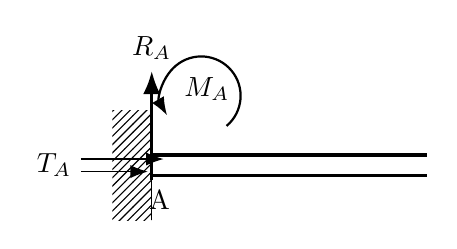
\begin{tikzpicture}[>=Latex]
  \fill[pattern=north east lines] (-0.5,-0.7) rectangle (0,0.7); \draw (0,-0.7) -- (0,0.7);
  \draw[line width=1.2pt] (0,0.13) -- (3.5,0.13);
  \draw[line width=1.2pt] (0,-0.13) -- (3.5,-0.13);
  \draw[->,very thick] (0,-0.18) -- (0,1.2) node[above]{$R_A$};
  \draw[->,thick] (0.95,0.5) arc (-50:210:0.5); \node[above] at (0.7,0.7) {$M_A$};
  \draw[-{Latex[length=2.2mm]}] (-0.9,0.08) -- (0.15,0.08);
  \draw[-{Latex[length=2.2mm]}] (-0.9,-0.08) -- (-0.05,-0.08);
  \node[left] at (-0.9,0) {$T_A$};
  \node[below] at (0.1,-0.2) {A};
\end{tikzpicture}
\end{center}

\[
  \ans{\;R_A = P\ (\text{上向き}),\qquad M_A = 2PL - M_C,\qquad T_A = T_B\;}
\]
検算：A まわりの曲げモーメントのつり合い $M_A + M_C - 2PL = (2PL-M_C)+M_C-2PL = 0$ ✓．

\medskip
\noindent\textbf{(2)}\quad トルクは B のトルクが全長に一様に伝わるので
\[
  T(x) = T_B \qquad (0\le x\le 2L).
\]
曲げモーメントは断面の右側にある荷重から求める．$M_C$ は C（$x=L$）で作用するから区間で分ける．\\
区間 CB（$L\le x\le 2L$）：右側には $P$ のみがあり, 下向き荷重なので
\[
  M(x) = -P(2L-x).
\]
区間 AC（$0\le x<L$）：右側に $P$ と $M_C$ があり
\[
  M(x) = -P(2L-x) + M_C .
\]
\[
  \ans{\;T(x)=T_B,\qquad
  M(x)=\begin{cases} -P(2L-x)+M_C & (0\le x<L)\\[2pt] -P(2L-x) & (L\le x\le 2L)\end{cases}\;}
\]
検算：$M(2L)=0$（自由端 B で 0）, $M(0)=M_C-2PL=-M_A$（支持モーメントに符号反転で一致）✓．

\medskip
\noindent\textbf{(3)}\quad 点 D は $x=L/2$ で区間 AC にあるから
\[
  M_D = M\!\left(\tfrac{L}{2}\right) = -P\!\left(2L-\tfrac{L}{2}\right)+M_C = M_C - \frac{3PL}{2}.
\]
最外縁 $z=d/2$ の曲げ応力は $\sigma_x=\dfrac{M_D\,(d/2)}{I}$, $I=\dfrac{\pi d^4}{64}$ より
\[
  \sigma_x = \frac{M_D\,(d/2)}{\pi d^4/64} = \frac{32 M_D}{\pi d^3}
           = \frac{32}{\pi d^3}\left(M_C-\frac{3PL}{2}\right).
\]
軸方向のみの曲げなので軸直交方向には垂直応力が生じず $\sigma_y=0$．
せん断応力はトルクによるねじり応力で, $\tau=\dfrac{T_B\,(d/2)}{J}$, $J=\dfrac{\pi d^4}{32}$ より
（最外縁では横荷重 $P$ による曲げせん断応力は 0）
\[
  \tau_{xy} = \frac{T_B\,(d/2)}{\pi d^4/32} = \frac{16 T_B}{\pi d^3}.
\]
\[
  \ans{\;\sigma_x = \dfrac{32}{\pi d^3}\!\left(M_C-\dfrac{3PL}{2}\right),\qquad
        \sigma_y = 0,\qquad \tau_{xy} = \dfrac{16 T_B}{\pi d^3}\;}
\]
検算：$\sigma_x=\dfrac{32M_C}{\pi d^3}-\dfrac{48PL}{\pi d^3}$, ねじり応力は曲げ応力の係数 $32/\pi d^3$ の半分
$16/\pi d^3$（$J=2I$ による）で整合 ✓．

\medskip
\noindent\textbf{(4)}\quad たわみの基礎式 $EI\,v''=M(x)$ を区間ごとに積分する．境界条件は固定端 A で
$v(0)=0,\ v'(0)=0$．\\
区間 AC（$M=Px+M_C-2PL$）：
\[
  EI\,v_1' = \frac{P}{2}x^2 + (M_C-2PL)x,\qquad
  EI\,v_1 = \frac{P}{6}x^3 + \frac{M_C-2PL}{2}x^2 .
\]
区間 CB（$M=Px-2PL$）：
\[
  EI\,v_2' = \frac{P}{2}x^2 - 2PL\,x + C_3,\qquad
  EI\,v_2 = \frac{P}{6}x^3 - PL\,x^2 + C_3 x + C_4 .
\]
接続条件 $v_1'(L)=v_2'(L),\ v_1(L)=v_2(L)$ より
\[
  C_3 = M_C L,\qquad C_4 = -\frac{M_C L^2}{2}.
\]
自由端 B（$x=2L$）では
\[
  EI\,v_2(2L) = \frac{P}{6}(2L)^3 - PL(2L)^2 + M_C L(2L) - \frac{M_C L^2}{2}
              = \frac{3M_C L^2}{2} - \frac{8PL^3}{3}.
\]
$v$ は下向きを正にとったから, 下向きのたわみ $\delta_B$ は上式の符号を反転して
\[
  \ans{\;\delta_B = \frac{1}{EI}\left(\frac{8PL^3}{3} - \frac{3M_C L^2}{2}\right)\ (\text{下向き正})\;}
\]
ねじれ角は $\psi_B = \dfrac{T_B\,(2L)}{G J}$, $J=\dfrac{\pi d^4}{32}$ より
\[
  \ans{\;\psi_B = \frac{2T_B L}{G J} = \frac{64\,T_B L}{\pi G d^4}\;}
\]
検算：$M_C=0$ のとき $\delta_B=\dfrac{8PL^3}{3EI}=\dfrac{P(2L)^3}{3EI}$ となり,
長さ $2L$ の片持ちはり先端集中荷重のたわみ公式に一致する ✓．

\medskip
\noindent\textbf{(5)}\quad $\delta_B=0$ より
\[
  \frac{8PL^3}{3} - \frac{3M_C L^2}{2} = 0
  \;\Longrightarrow\;
  M_C = \frac{8PL^3}{3}\cdot\frac{2}{3L^2}.
\]
\[
  \ans{\;M_C = \frac{16PL}{9}\;}
\]
検算：$\dfrac{3}{2}\cdot\dfrac{16PL}{9}\,L^2=\dfrac{8PL^3}{3}$ となり $P$ による下向きたわみを打ち消す ✓．

\end{document}
